\cleardoublepage
\chapterimage{bg/10}

\chapter{Valorisation d'Inforsid}


	\section{Présentation du contexte}
		Depuis sa création en 1983 le congrès Inforsid réunit chaque année les chercheurs travaillant dans le domaine de l'informatique des organisations. Il se tient chaque année dans une ville différente, et chaque édition dispose de son propre comité de programme. Ce comité est constitué d'un ou plusieurs président(es) ayant pour premières tâches de choisir le reste des membres et occasionnellement des adjoint(e)s.
	
		Tout ceci représente une masse d'information non négligeable, rassemblée pour chaque congrès dans un ouvrage : les actes du congrès. Cependant la recherche d'une information particulière dans ces ouvrages peut être laborieuse (participation d'un chercheur à une édition ou chercheurs les plus impliqués dans le comité de programme par exemple).
		
		Pour pallier ce problème Guillaume Cabanac et Marc Ternisien ont mis en place en 2010 une base de données Oracle et une application web\footnote{Consultable à l'adresse \url{http://www.irit.fr/~Guillaume.Cabanac/inforsid}.} centralisant ces informations. Celles-ci permettent, pour chaque édition du congrès, de visualiser son comité de programme et la liste des articles présentés avec leurs auteurs respectifs. L'application web comporte également une «~fiche de présentation~» pour chaque chercheur ayant participé à Inforsid au cours des années. Cette fiche permet de voir :
		\begin{itemize}
			\item la liste des articles présentés par le chercheur en question,
			\item ses participations au comité de programme,
			\item sa localisation au cours des années (déterminée grâce à ses différentes participations au comité de programme et aux articles qu'il a présentés),
			\item les chercheurs avec qui il a écrit des articles présentés au congrès (avec la(les) année(s) de collaboration).
		\end{itemize}
		
		Une autre fonctionnalité est également présente dans l'application : la suggestion de membres pour la constitution du comité de programme. En effet, jusqu'alors les présidents n'avaient aucune règle ou aide pour sélectionner d'éventuels membres. Ils devaient donc se fier à leur connaissance de la communauté. Cela pouvait entraîner l'oubli de certains membres de la communauté, ou la favorisation de certains. La suggestion de membres via l'application se base sur un algorithme et permet une constitution plus éclairée, tout en s'assurant de n'oublier aucun chercheur. L'algorithme liste les chercheurs :
		\begin{itemize}
			\item ayant présenté au moins un article lors d'un congrès depuis 2005, 
			\item ayant écrit au moins 2 articles,
			\item n'ayant jamais fait partie d'un comité de programme (ceux-ci étant favorisés) ou en ayant fait partie avant 2008.
		\end{itemize}
		
		Mon travail consistait à intégrer dans cette application les données des congrès Inforsid 2012 et 2013 et de valoriser le congrès.
		

	\section{Intégration des données des éditions 2012 et 2013}
		La transformation des données pour leur insertion dans la base de données se faisait par l'intermédiaire d'un programme en C, dont je devais donc comprendre le fonctionnement. Heureusement Marc Ternisien, le stagiaire ayant initialement développé l'application, avait fourni une documentation claire qui m'a permis de rapidement prendre en main l'application et d'insérer les données des éditions 2012 et 2013 sans souci.
		
		
			\subsection{Principe de la transformation des données}
				Les données générales des congrès sont présentes dans un fichier texte contenant, pour chaque édition, une ligne de la forme «~\texttt{année, ville}~».
				Les informations détaillées se trouvent dans 2 fichiers texte placés dans un répertoire nommé selon l'année concernée~:
				\begin{itemize}
					\item un fichier contenant les membres du comité de programme,
					\item un fichier contenant les articles présentés durant le congrès avec leurs auteurs.
				\end{itemize}
				
				Une fois les données dans ces fichiers, l'application C crée les fichiers destinés à être insérés dans la base de données construite selon le MCD présenté en figure~\ref{fig:mcd}. La structure des fichiers est présentée dans le tableau~\ref{tab:struct}.
				
				\begin{savenotes}%pour voir les footnote du tabular
				\begin{table}[h]
					\centering
					\caption{Structure des fichiers destinés à être insérés dans la base de données}\label{tab:struct}
					\begin{tabular}{ll}
						&\\
						\toprule
						\textit{Fichier} & \textit{Structure}\\
						\midrule
						article.txt		& \texttt{idArticle;titre;année;} \\
						congres.txt	& \texttt{année;idVille;} \\
						personne.txt	& \texttt{idPersonne;prénom;nom;} \\
						ville.txt		& \texttt{idVille;nomVille;paysVille;} \\
						ecrire.txt		& \texttt{idArticle;idPersonne;idVille;rang\footnote{Position à laquelle la personne apparaît lors de la déclaration des coauteurs dans l'article.}} \\
						membre.txt	& \texttt{idPersonne;année;rôle\footnote{Président(e) = \lq{}P', membre = \lq{}M' ou adjoint(e) = \lq{}A'};idVille} \\
						\bottomrule
						&\\
					\end{tabular}
				\end{table}
				\end{savenotes}
				
				\begin{figure}[h]
					\center
					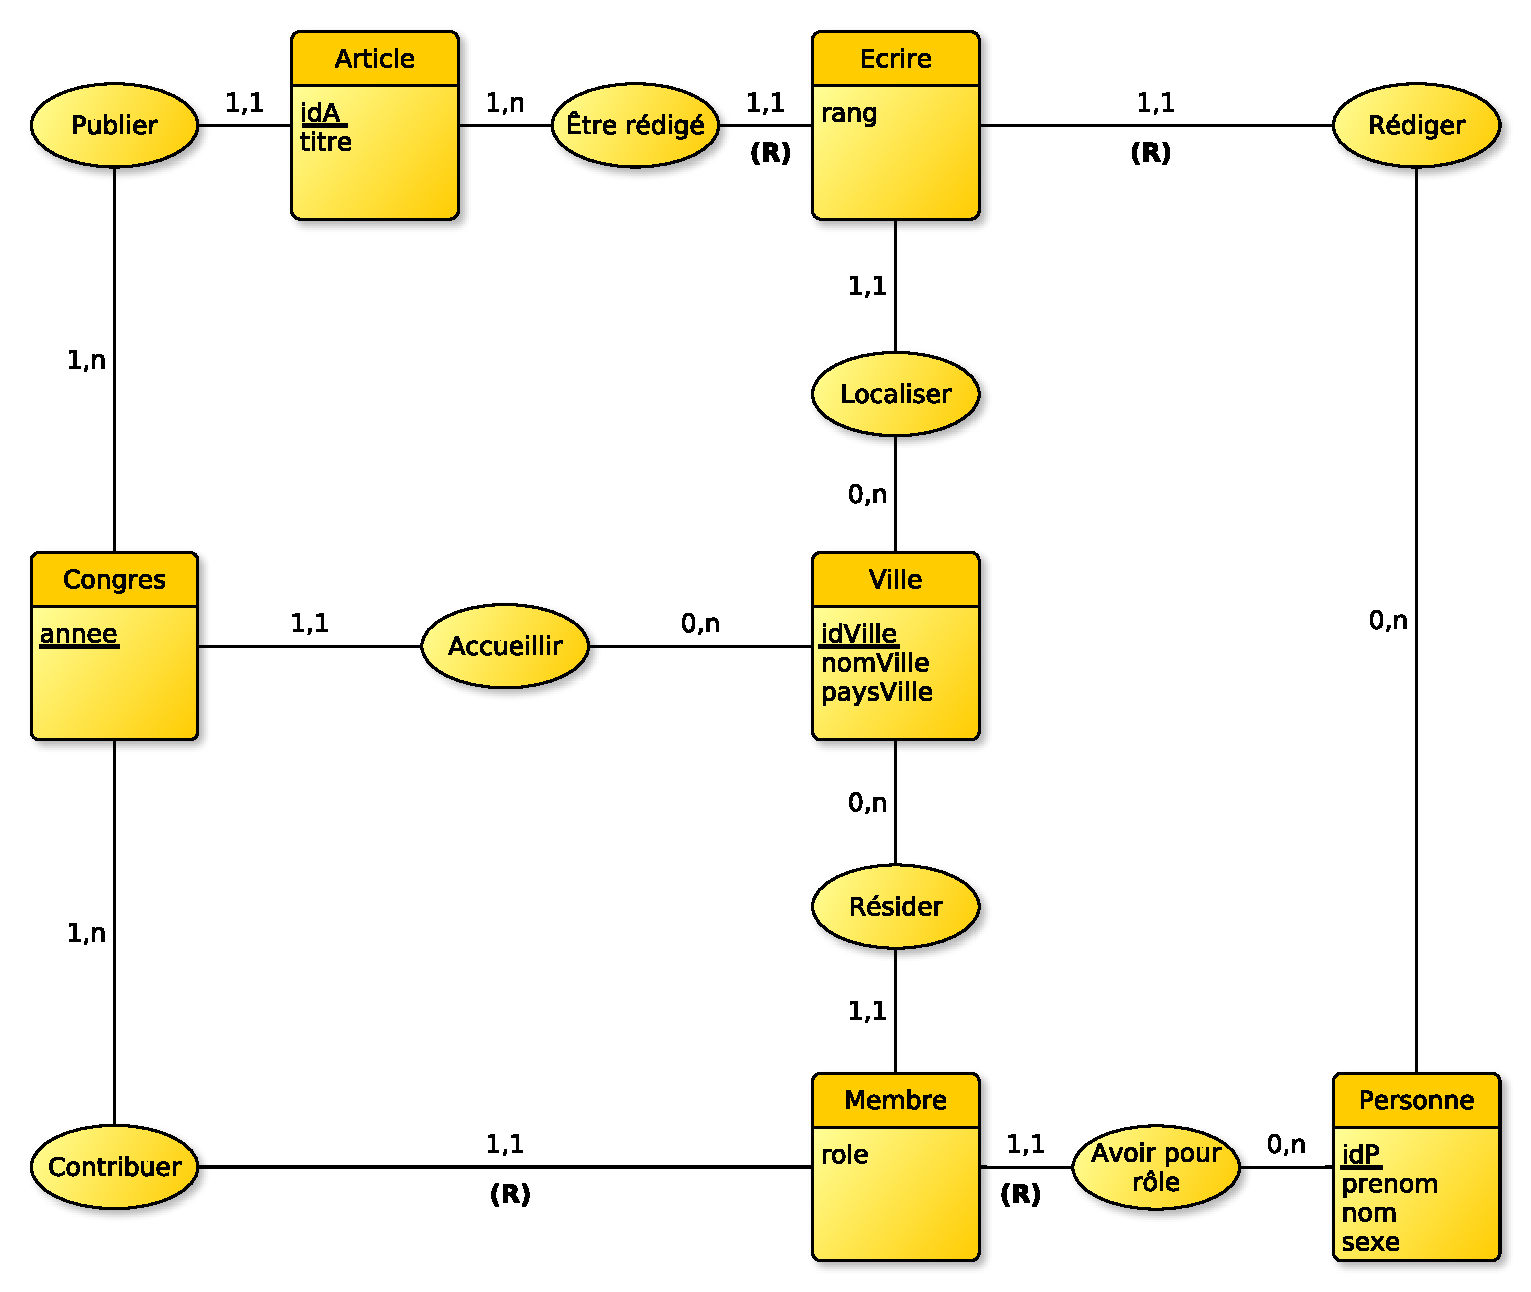
\includegraphics[width=\textwidth]{ch5/inforsid/mcd}
					\caption{Modèle Conceptuel de Données de la base utilisée par l'application \citep{ternisien}}\label{fig:mcd}
				\end{figure}
	
				Par défaut le pays était placé à «~FRANCE~» mais il existait 2 méthodes pour corriger ceci avant l'insertion des données dans la base :
				\begin{itemize}
					\item l'utilisateur pouvait modifier la valeur directement dans le fichier \texttt{ville.txt} généré précédemment,
					\item s'il existait déjà un fichier \texttt{ville.txt} lorsque le programme de transformation de données était exécuté, celui-ci récupérait les pays attribués aux villes présentes dans ce fichier.
				\end{itemize}
	
	
			\subsection{Améliorations apportées au processus d'intégration des données}			
		
		\subsubsection{Gestion des «~synonymes~»}
			Un des problèmes de la méthode d'insertion des données de l'application était qu'il était très difficile de repérer une faute de frappe avant l'insertion des données dans la base. En effet, celles-ci étant dispersées dans de nombreux fichiers, il aurait été fastidieux de tous les contrôler à la recherche d'éventuelles erreurs. Or il existait de nombreux cas de noms de villes ou de personnes «~synonymes~», tels que «~Sophia~Antipolis~» et «~Sophia-Antipolis~» ou «~Cauvet~Corine~» et «~Cauvet~Corinne~».
			
			Pour résoudre ce problème, j'ai mis en place une méthode de détection des synonymes simple et pratique pour l'utilisateur. Celui-ci devait simplement supprimer d'une liste les couples de synonymes détectés par erreur puis lancer une procédure qui prenait en charge la «~fusion~» des deux entités.
			
			Cette méthode est présentée plus en détail dans les annexes.
			 
			 
		\subsubsection{Gestion des pays}
			Les pays correspondant aux villes présentes dans la base devaient avant être précisés manuellement dans un fichier texte, et la méthode de récupération des pays insérés précédemment présente dans le programme en C déclenchait souvent des erreurs.
			
			J'ai donc décidé d'automatiser au maximum la procédure. J'ai ajouté à la base de données une table contenant de nombreux couples «~Ville - Pays~» et mis en place une procédure mettant à jour les villes d'Inforsid à partir de ceux-ci. Si, après une insertion de données, l'une des villes n'était pas présente dans la table de référence elle apparaissait dans une vue où l'utilisateur pouvait préciser manuellement son pays. Il n'avait ensuite qu'à relancer la procédure.
			
			L'avantage de cette méthode est que la base de villes présentes  -- et donc automatiquement gérées -- augmente d'année en année, au fur et à mesure des insertions de données.
	

	\section{Valorisation du congrès}
	
		\subsection{Pôles principaux}
			Afin de montrer les pôles principaux d'Inforsid, j'ai calculé le poids de chaque ville impliquée dans le congrès. Ce calcul repose sur les articles présentés lors des éditions du congrès et est défini comme suit :
			\begin{itemize}
				\item à chaque article est attribué un poids de 1,
				\item ce poids est attribué à la ville de rattachement que l'auteur indique dans son article,
				\item si l'article est rédigé par plusieurs auteurs, alors ce poids est réparti équitablement entre tous les auteurs (et donc entre leurs villes de rattachement).
			\end{itemize}
		
			J'ai tout d'abord souhaité proposer une visualisation nationale d'Inforsid. Pour cela j'ai sélectionné les 20 villes françaises ayant les poids les plus importants et je les ai représentées sur un fond de carte en utilisant des ronds dont la taille est proportionnelle au poids. Le résultat est visible sur la figure~\ref{fig:fr}.
			
			\begin{figure}[h]
				\centering
				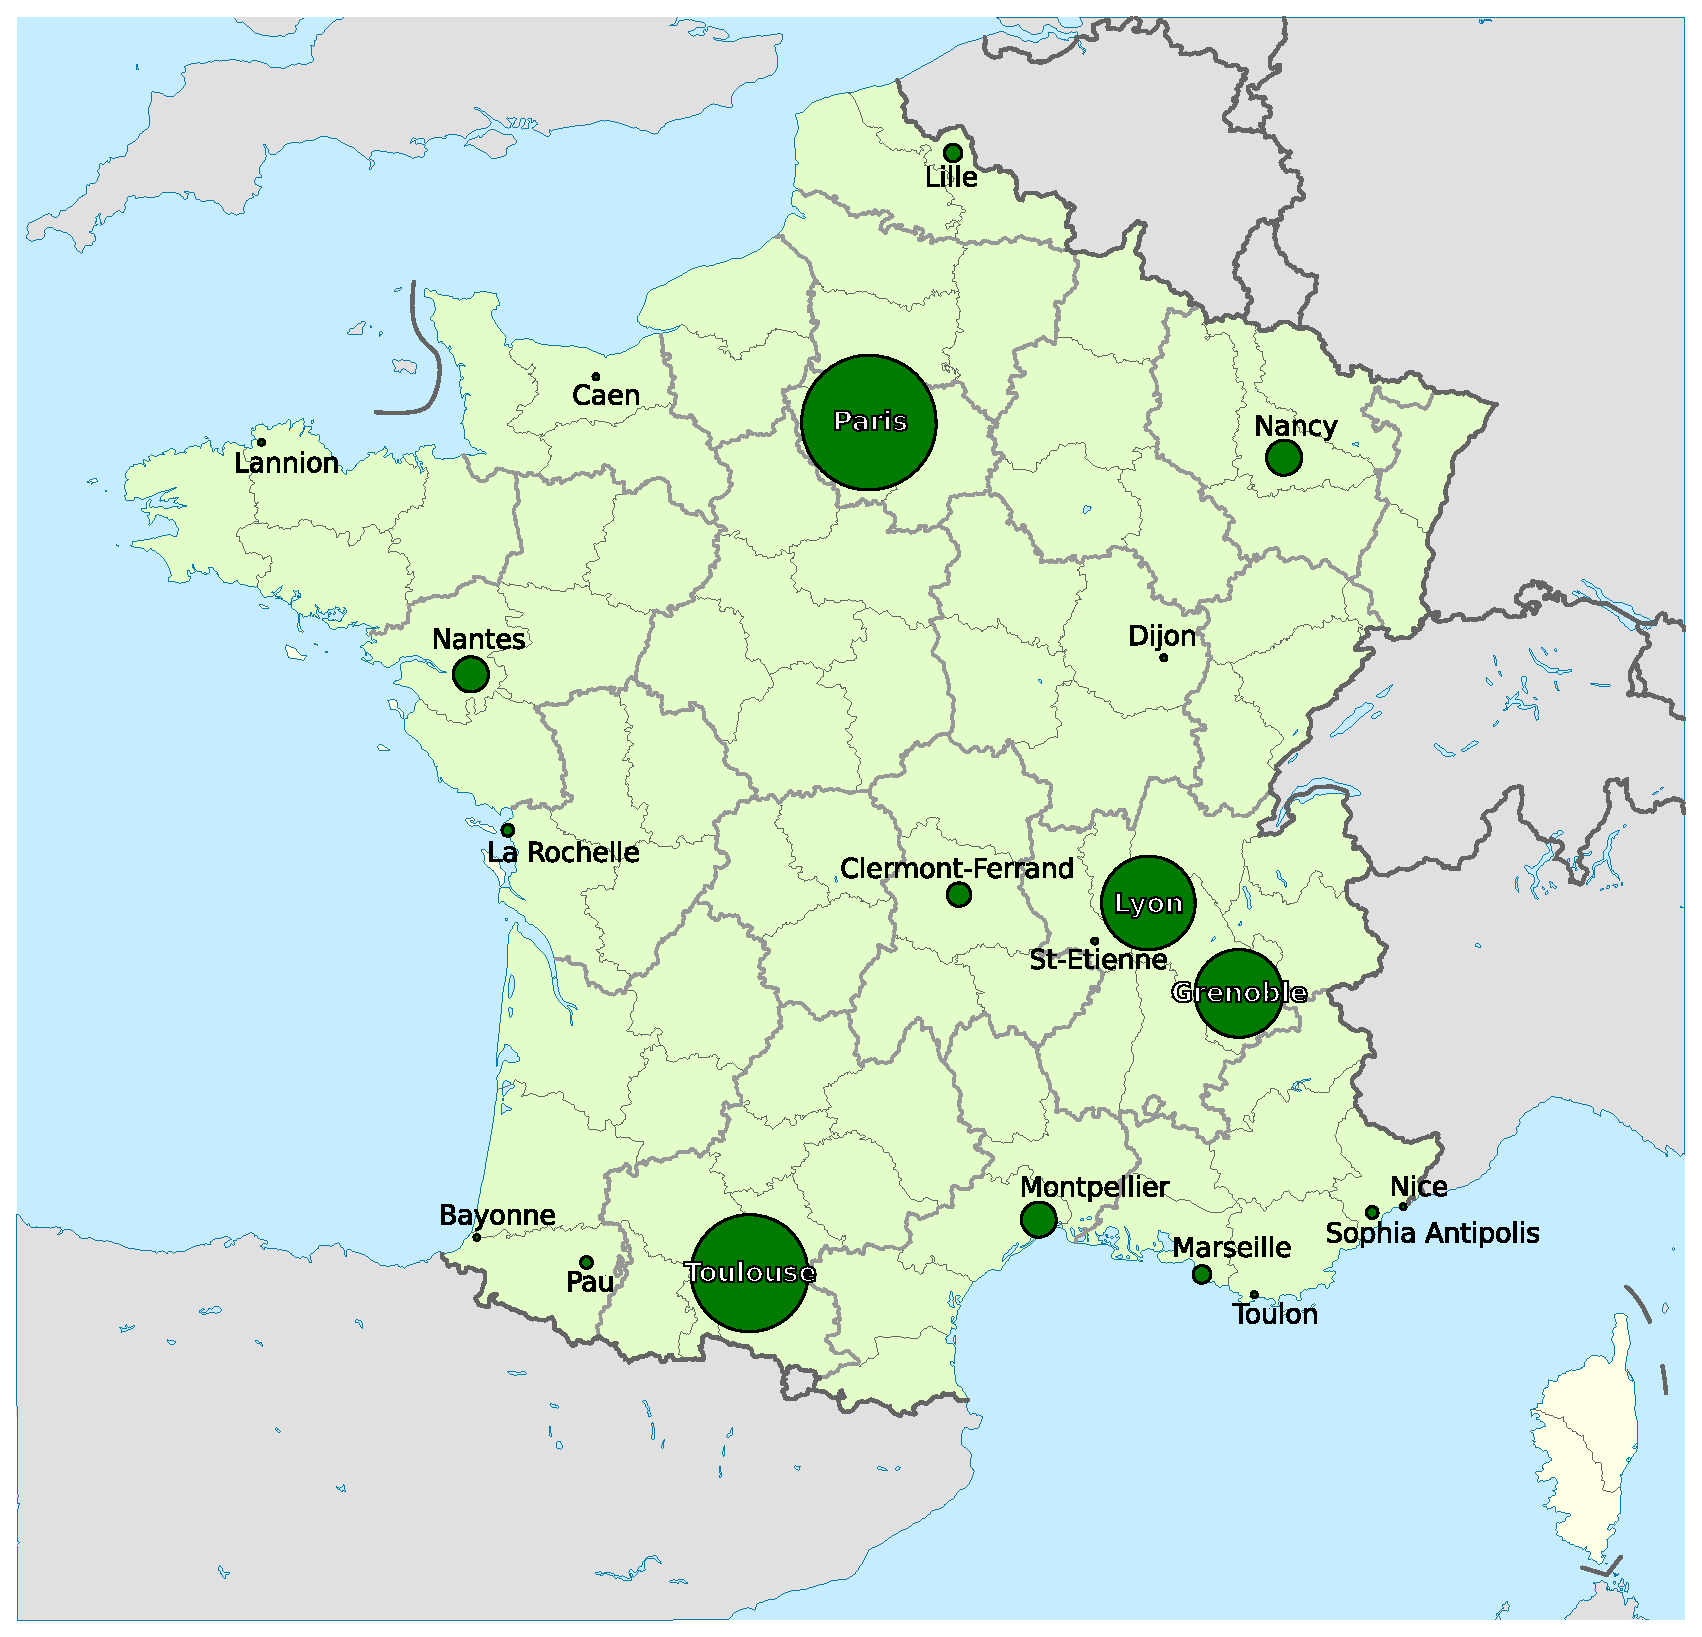
\includegraphics[width=\textwidth]{ch5/inforsid/fr.pdf}
				\caption{Les 20 villes françaises les plus présentes dans les affiliations des auteurs d'Inforsid}\label{fig:fr}
			\end{figure}
		
			Inforsid étant un congrès francophone réunissant des chercheurs de diverses nationalités différentes, j'ai ensuite souhaité représenter son rayonnement international. Pour cela j'ai utilisé les poids des pays --~calculés en additionnant les poids de leurs villes~-- qui m'ont permis de définir une «~échelle de teinte~»~: plus le pays était vert plus il était impliqué dans Inforsid.
			
			J'avais commencé à travailler sur une mappemonde, mais la majorité des pays participants étant en Europe, la lisibilité était bien trop mauvaise. Guillaume Cabanac avait alors suggéré que j'utilise à la place une carte de l'Europe et que je fasse figurer les pays n'y apparaissant pas sous forme de ronds de tailles différentes à coté (en utilisant la même méthode que celle utilisée pour représenter les villes). Le résultat est présenté en figure~\ref{fig:eu}.
			
			\begin{figure}[h]
				\centering
				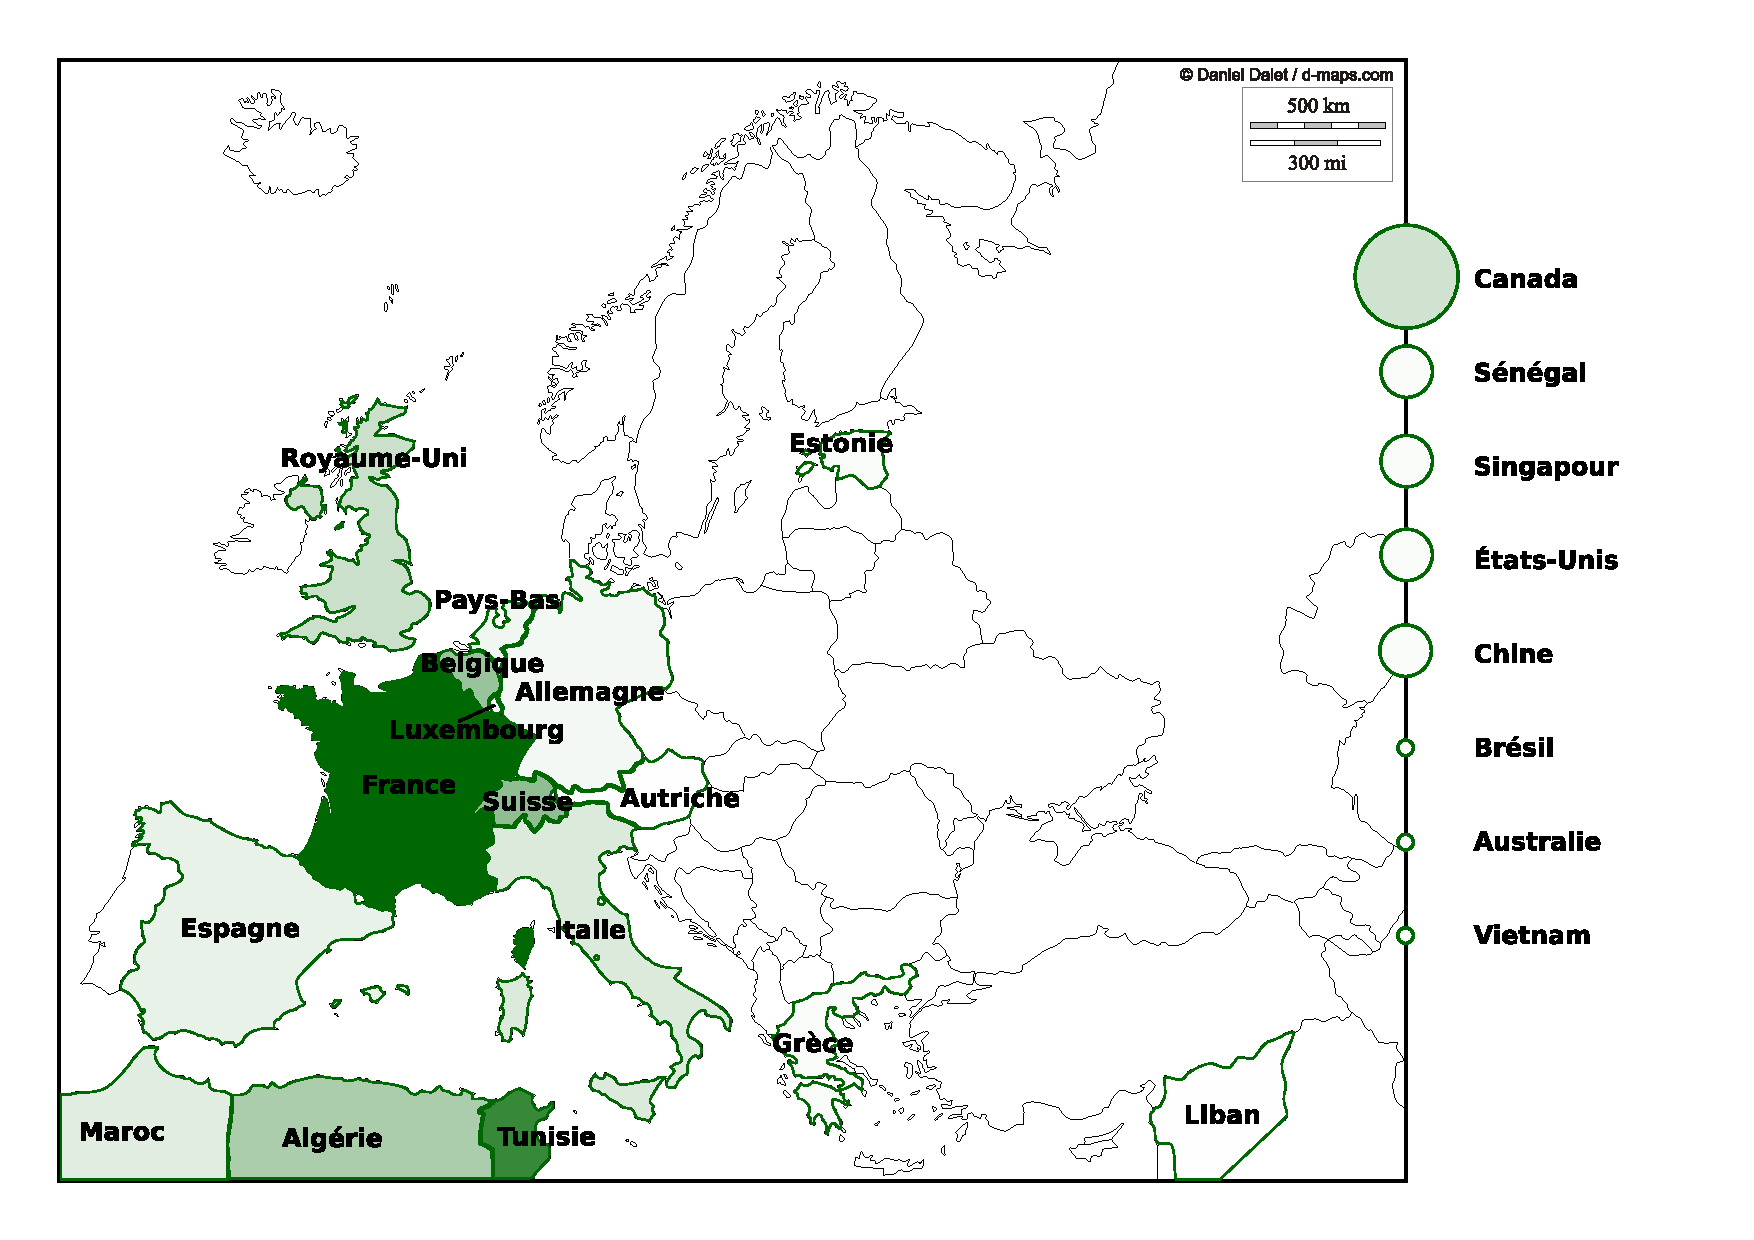
\includegraphics[width=\textwidth]{ch5/inforsid/eu.pdf}
				\caption{Les pays des auteurs publiant à Inforsid}\label{fig:eu}
			\end{figure}
			
			
		\subsection{Thèmes du congrès}
			Afin de valoriser d'Inforsid il a été décidé de représenter l'évolution des thèmes traités par le congrès. Pour illustrer cela je devais réaliser des nuages de mots à l'aide de Wordle\footnote{\url{http://www.wordle.net/}}.
			
			Pour évaluer les thèmes abordés j'ai pris comme source d'information les termes employés dans les titres des articles présentés. Ces termes étaient «~normalisés~» afin de réaliser des calculs pertinents~: suppression des accents, des caractères spéciaux et des «~s~» finaux. J'ai donc créé trois vues associant à chaque terme son nombre d'occurrences selon une période donnée :
			\begin{itemize}
				\item la première comptait les occurrences des mots des éditions du congrès jusqu'en 1993,
				\item la seconde comptait les occurrences des mots de 1994 à 2003,
				\item la troisième comptait les occurrences des mots de 2004 à 2013.
			\end{itemize}
			
			Je me suis limitée aux 50 termes les plus fréquents afin de ne pas surcharger les nuages de mots et ainsi faciliter leur lecture --~les mots vides n'étaient bien entendu pas compris parmi ceux-ci. J'ai ainsi obtenu les nuages de mots présentés en figures~\ref{fig:n1}, \ref{fig:n2} et \ref{fig:n3}.
			
			\begin{figure}[p]
				\centering
				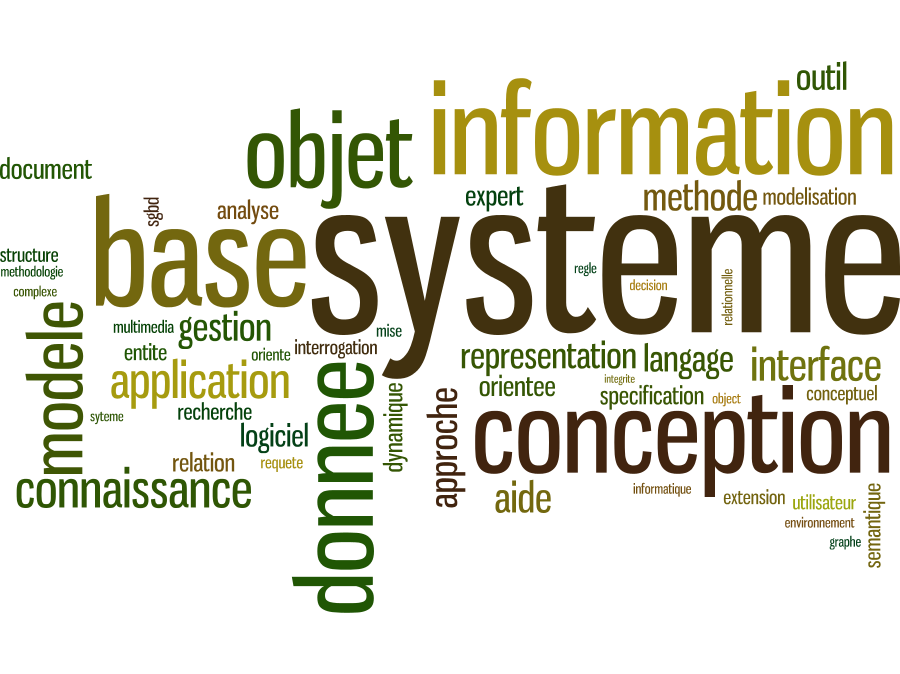
\includegraphics[width=0.6\textwidth, height=0.4\textwidth]{ch5/inforsid/w1}
				\caption{Termes représentant Inforsid de 1983 à 1993}\label{fig:n1}
			\end{figure}
			
			\begin{figure}[p]
				\centering
				
\includegraphics[width=0.6\textwidth, height=0.4\textwidth]{ch5/inforsid/w2}
				\caption{Termes représentant Inforsid de 1994 à 2003}\label{fig:n2}
			\end{figure}
			
			\begin{figure}[p]
				\centering
				
\includegraphics[width=0.6\textwidth, height=0.4\textwidth]{ch5/inforsid/w3}
				\caption{Termes représentant Inforsid de 2004 à 2013}\label{fig:n3}
			\end{figure}
		
			Cependant ces nuages de mots avaient une faiblesse : ils ne prenaient pas en compte les expressions de deux ou trois mots. Pour pallier ce problème j'ai créé une procédure PL/SQL détectant toutes ces expressions. Il a ensuite fallu que je fasse un filtrage manuel dans la table afin de ne garder que les expressions pertinentes pour nous, puis que j'uniformise les poids des mots en fonction des expressions conservées. En effet les poids des termes présents dans ces expressions devaient être diminués afin de ne pas fausser les résultats -- par exemple «~donnee~» étant présent dans «~base de donnee~» il fallait ôter de son poids le poids de l'expression. J'ai ainsi obtenu les wordles présents dans les figures~\ref{fig:w4}, \ref{fig:w5} et \ref{fig:w6}.
		
			\begin{figure}[p]
				\centering
				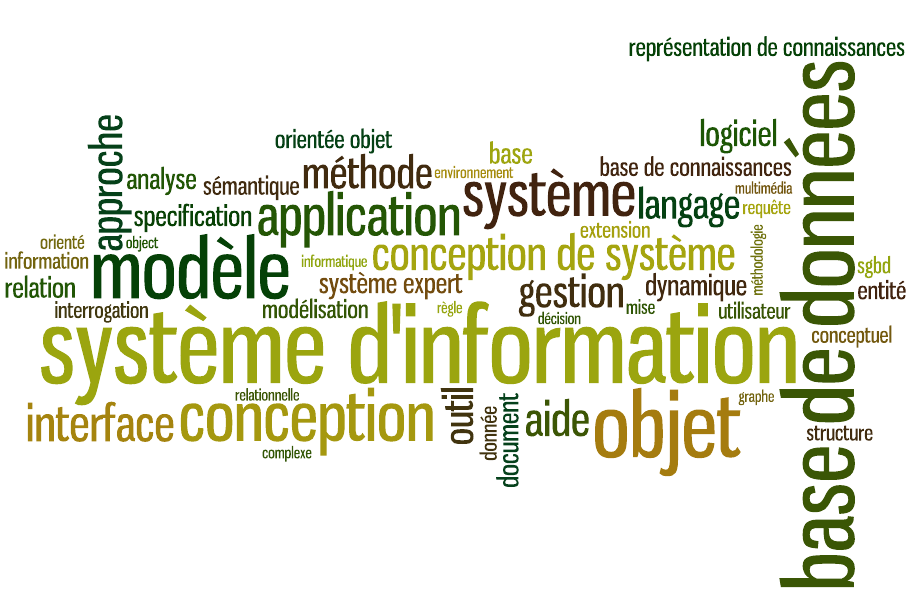
\includegraphics[width=0.6\textwidth]{ch5/inforsid/w4}
				\caption{Termes représentant Inforsid de 1983 à 1993 en prenant en compte les expressions}\label{fig:w4}
			\end{figure}
		
			\begin{figure}[p]
				\centering
				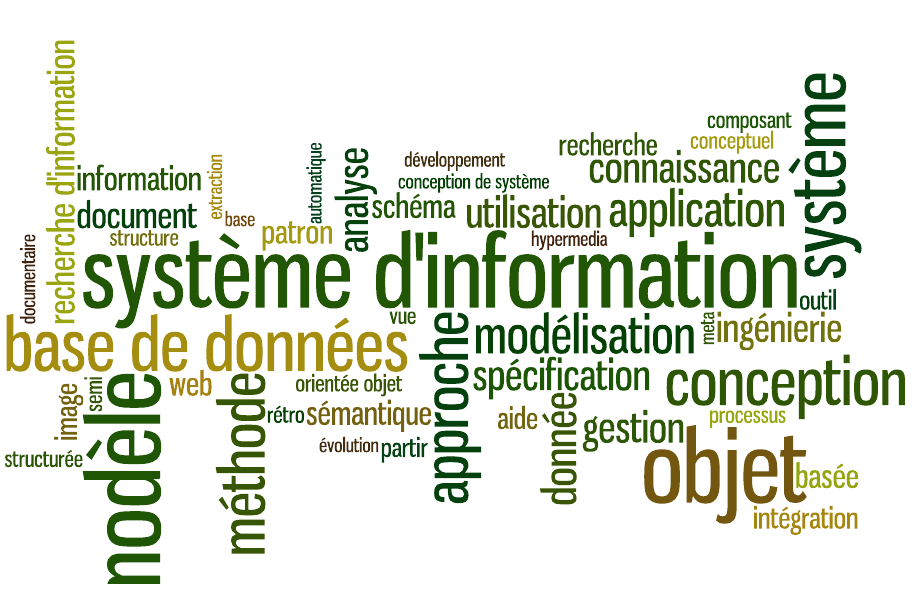
\includegraphics[width=0.6\textwidth]{ch5/inforsid/w5}
				\caption{Termes représentant Inforsid de 1994 à 2003 en prenant en compte les expressions}\label{fig:w5}
			\end{figure}
		
			\begin{figure}[p]
				\centering
				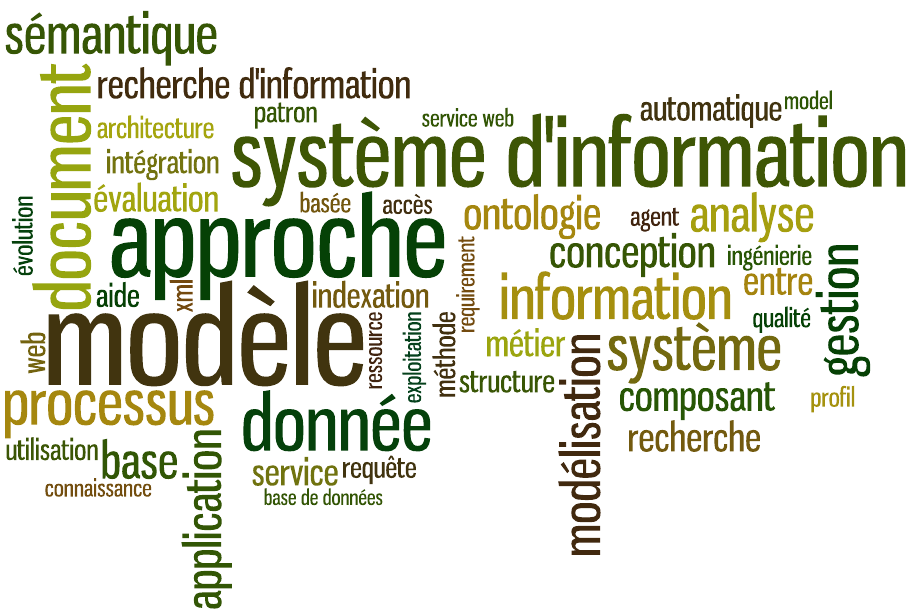
\includegraphics[width=0.6\textwidth]{ch5/inforsid/w6}
				\caption{Termes représentant Inforsid de 2004 à 2013 en prenant en compte les expressions}\label{fig:w6}
			\end{figure}
	
	
		\subsection{Influence des membres}
			Je devais identifier les chercheurs participant à Inforsid qui sont membres de comités de rédaction de journaux scientifiques du domaine IS. Au moment où j'ai eu à réaliser cette tâche je disposais de la base \texttt{cabanac\_dblp2013}, contenant notamment les comités de rédaction des 77 journaux traités dans \citep{shaping} (pour plus d'informations, voir le chapitre \ref{cha:genre}). J'ai donc calculé l'intersection entre les membres d'Inforsid et les membres de comités de rédaction présents dans DBLP . Les chercheurs obtenus sont présentés dans le tableau~\ref{tab:boards}.
		
			\begin{table}[p]
				\centering
				\caption{Membres d'Inforsid membres de comités de rédaction de journaux scientifiques du domaine IS}\label{tab:boards}
				\input{tableaux/ch5/inforsid/board}
			\end{table}
			
			J'ai ensuite mis en valeur sur la carte les journaux trouvés. La carte finale est visible en figure~\ref{fig:map}. On constate que la majorité des journaux mis en valeur sont dans la partie supérieure gauche de la carte, soulignant une similarité des thèmes traités.
			
			\begin{figure}[ht]
				\centering
				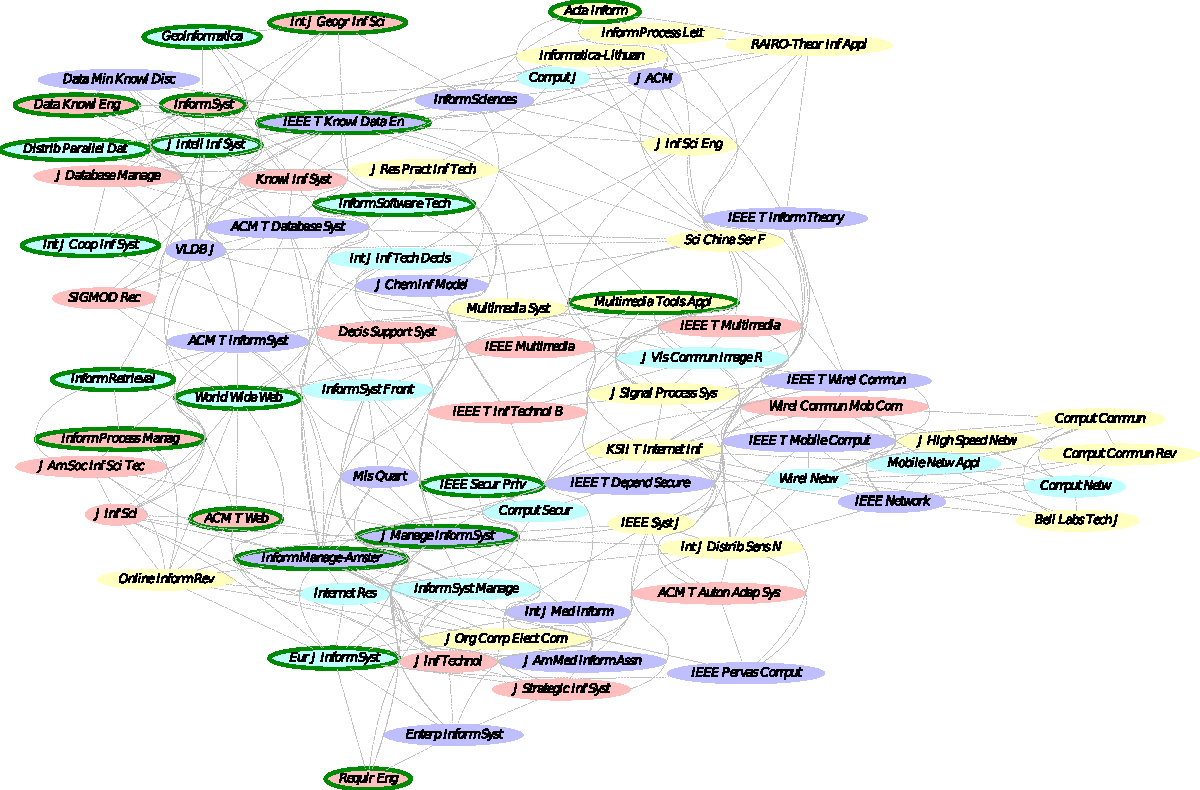
\includegraphics[width=\textwidth]{ch5/inforsid/map}
				\caption{Cartes des 77 principaux journaux du domaine IS \citep{shaping}. Les journaux ayant des comités de rédaction auxquels participent des membres d'Inforsid sont repérés par un liséré vert}\label{fig:map}
			\end{figure}
		
		
		\subsection{Villes ayant accueilli le congrès}
			Les retours des utilisateurs sur notre site web présentant Inforsid ont montré qu'il pourrait être pertinent de réaliser une carte montrant où les congrès avaient eu lieu, afin de montrer le fait qu'il s'agissait bien d'un congrès national. La carte réalisée est visible dans la figure~\ref{fig:mapVilles}.
			
			\begin{figure}[h]
				\centering
				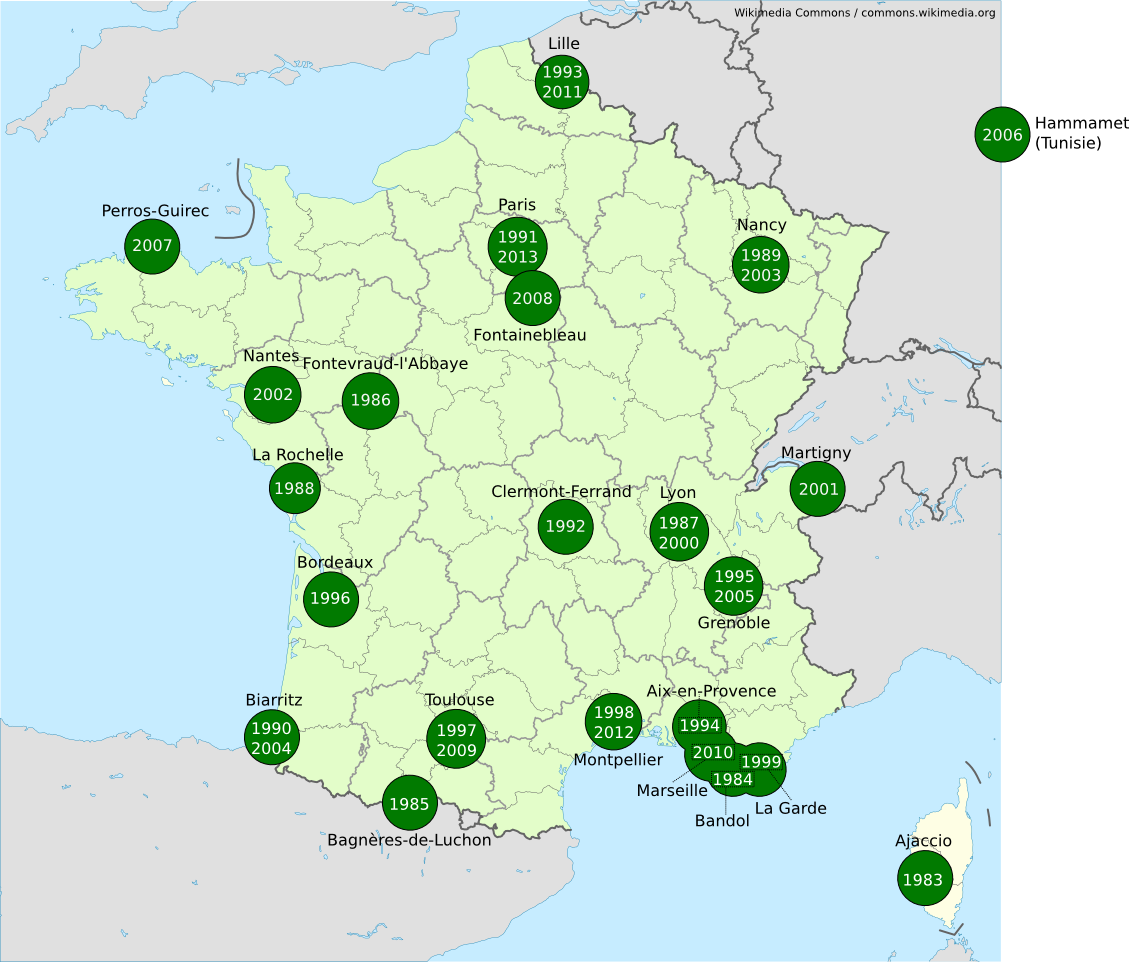
\includegraphics[width=\textwidth]{ch5/inforsid/mapVilles}
				\caption{Villes ayant accueilli le congrès Inforsid}\label{fig:mapVilles}
			\end{figure}
	
	\section{Modification du site web}
			
		\subsection{Optimisation des procédures PL/SQL}
			L'application web était constituée de 6 procédures :
			\begin{itemize}
				\item \texttt{Inforsid\_Accueil} affichait la page d'accueil permettant d'accéder aux résumés des différentes éditions du congrès, de rechercher un chercheur ou d'accéder aux suggestions pour le comité de programme.
				\item \texttt{Inforsid\_Fiche\_Annee} affichait le résumé d'une édition.
				\item \texttt{Inforsid\_Statut\_Personne} affichait le résumé du chercheur.
				\item \texttt{Inforsid\_Traitement} recherchait un chercheur dans la base et affichait la liste des personnes trouvées ou directement la fiche du chercheur s'il n'y avait qu'un seul résultat.
				\item \texttt{Inforsid\_Suggestions\_CP} affichait la liste des membres proposés par le système pour la constitution du comité de programme
				\item \texttt{Inforsid\_Footer} affichait le pied-de-page X/HTML.
			\end{itemize}

			Afin d'améliorer la qualité du code, j'ai pour ma part réorganisé le code de chaque procédure afin d'avoir le plus possible la structure suivante : récupération puis affichage des données. De plus, afin de diminuer les répétitions de code, j'ai créé 2 nouvelles procédures :
			\begin{itemize}
				\item \texttt{Inforsid\_Header} affichant l'en-tête X/HTML des pages avec les titres passés en paramètre (un paramètre pour le titre de la page affichée par le navigateur et un pour le titre principal \texttt{<h1>} affiché dans la page).
				\item \texttt{Inforsid\_Retour\_Accueil} affichant un lien permettant de retourner à l'accueil.
			\end{itemize}
			
			À la demande de Guillaume Cabanac j'ai également supprimé la mention de la personne ayant présenté le plus d'articles présente sur la page d'accueil et inversé l'ordre de présentation des participations au comité de programme et de sa localisation (présenté précédemment dans l'ordre chronologique et désormais du plus récent au plus ancien). J'ai également modifié le code afin de n'avoir à modifier qu'un seul élément lors d'une migration de l'application sur une nouvelle base de données, et non toutes les procédures.
			
			
		\subsection{Création d'une nouvelle charte graphique}
			Afin d'améliorer le site et de pouvoir utiliser les fonctionnalités HTML les plus récentes j'ai choisi de passer le site web en HTML5. Il a fallu pour cela que je modifie de nombreux éléments de style, qui n'étaient plus supportés par la dernière version de HTML, afin d'être conforme aux recommandations du W3C. Cette mise à niveau m'a permis d'utiliser Bootstrap\footnote{Bibliothèque CSS et Javascript éditée par Twitter.} afin de modifier le graphisme du site. Vous pouvez voir l'ancien graphisme sur la figure~\ref{fig:old} et le nouveau sur la figure~\ref{fig:new}.
			
			J'ai inséré sur la page d'accueil les graphiques réalisés (cartes et nuages de mots présentés tout au long de cette section) afin de permettre au visiteur de mieux connaître le congrès.
		
			J'ai également ajouté des liens vers les actes Inforsid\footnote{Présents à l'adresse \url{https://liris.cnrs.fr/inforsid/?q=Actes\%20Inforsid}}. Il aurait été préférable de faire un lien vers chaque article mais malheureusement nous n'avons pas trouvé de moyen pour réaliser ceci de manière automatique.
			
			\begin{figure}[p]
				\centering
				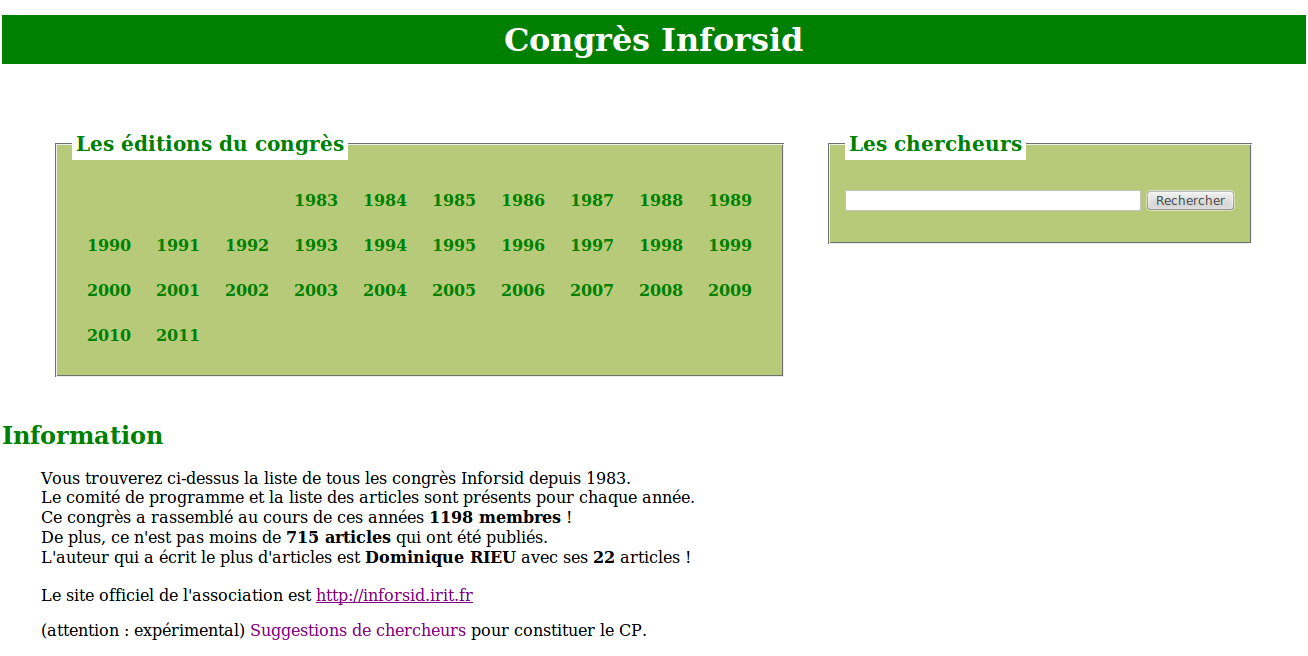
\includegraphics[width=0.9\textwidth]{ch5/inforsid/old}
				\caption{Ancien aspect du site web}\label{fig:old}
			\end{figure}
			
			\begin{figure}[p]
				\centering
				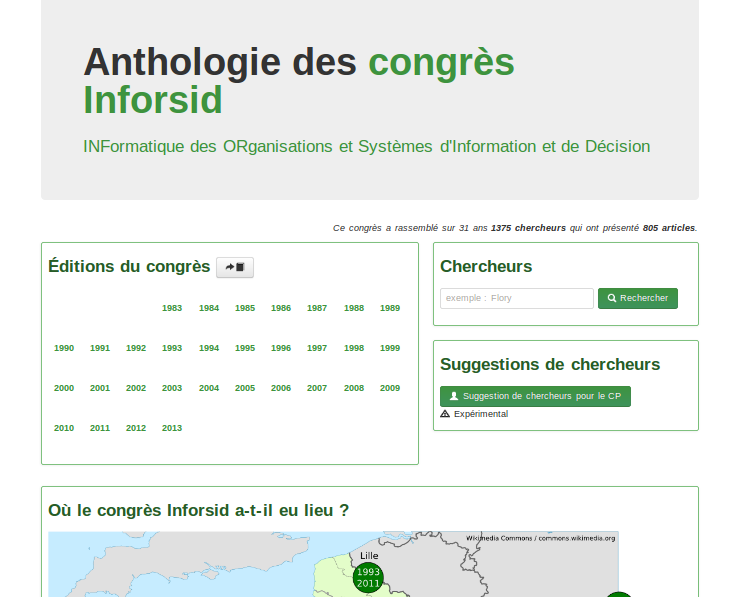
\includegraphics[width=0.9\textwidth]{ch5/inforsid/new}
				\caption{Nouvel aspect du site web}\label{fig:new}
			\end{figure}

